\documentclass[10pt]{article}

\usepackage{fullpage}
\usepackage{longtable}
\usepackage[pdftex]{graphicx}
\DeclareGraphicsExtensions{.pdf,.jpg}

% no numbers, etc
\pagestyle{empty}

\begin{document}

{\bf Homework 1} \hfill {\raggedleft Thomas Torsney-Weir}

%Each homework problem goes here
\begin{enumerate}
\item % formulating search
  \begin{enumerate}
  \item % stacking
    \begin{description}
    \item[Initial State]
      Stack of items of size 0 and self and all items in remaining set:
      $([], {I, F, C})$.
    \item[Goal Test]
      Sum of heights of items on stack is greater or equal to 9.
    \item[Successor]
      Remove item from top of stack or place one of remaining items on 
      top of stack.  If removing add item to set of available items.  If
      adding to stack then remove item from set of available items.
    \item[Cost Function]
      Cost to add or remove item from the top of the stack is 1.
    \end{description}
  \item % kevin bacon
    \begin{description}
    \item[Initial State]
      No actors named and $X$ contains all actors: $(\emptyset, X)$.
    \item[Goal Test]
      Successor function returns nothing and is the other player's turn.
    \item[Successor]
      Given an actor $a$, for each actor, $a'$ such that $a' \in X$ and $a'$
      is in a movie with $a$ return $(a', X / a')$.
    \item[Cost Function]
      Cost to name an actor is always 1.
    \end{description}
  \end{enumerate}
  
\item % blind search
  \begin{enumerate}
  \item % a
    \ \\
    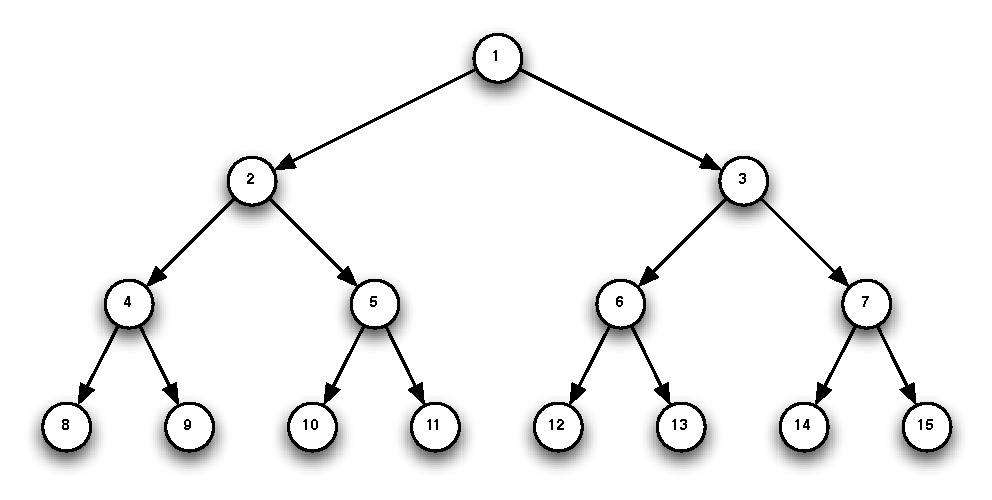
\includegraphics[width=5.5in]{2a_nextstates.pdf}
  \item % b
    \begin{description}
    \item[Bredth First Search]
      1, 2, 3, 4, 5, 6, 7, 8, 9, 10, 11
    \item[Depth-limited Search] % limit 3
      1, 2, 4, 8, 9, 5, 10, 11
    \item[IDS]
      1, 1, 2, 3, 1, 2, 3, 4, 5, 6, 7, 1, 2, 3, 4, 5, 6, 7, 8, 9, 10, 11
    \end{description}
  \end{enumerate}
\item % heuristic search
  \begin{enumerate}
  \item % uniform cost
    Uses graph search
    \begin{enumerate}
    \item % list of nodes generated
      \begin{tabular}[t]{|r|l|l|p{20em}|}
      \hline
      Step & Path & Visited            & Queue (path,$g$) \\
      \hline
      1    & S    & $\{S\}$                & $(SA,2),(SD,3)$ \\
      \hline
      2    & SA   & $\{S,A\}$              & $(SD,3),(SAS,4),(SAB,6),(SAD,7)$ \\
      \hline
      3    & SD   & $\{S,A,D\}$            & $(SAS,4),(SAB,6),(SAD,7), \linebreak
                                          (SDS,6), (SDA,8),(SDE,6)$ \\
      \hline
      4    & SAB  & $\{S,A,B,D\}$          & $(SAD,7),(SDS,6),(SDA,8), \linebreak
                                          (SDE,6),(SABA,10),(SABC,10), \linebreak
                                          (SABE,12), (SABF,9)$ \\
      \hline
      5    & SDE  & $\{S,A,B,D,E\}$        & $(SAD,7),(SDA,8),(SABA,10), \linebreak
                                          (SABC,10),(SABE,12),(SABF,9), \linebreak
                                          (SDED,9),(SDEF,10),(SDEB,12)$ \\
      \hline
      6    & SABF & $\{S,A,B,D,E,F\}$      & $(SABA,10),(SABC,10),(SABE,12), \linebreak
                                          (SDED,9),(SDEF,10),(SDEB,12), \linebreak
                                          (SABFG,14),(SABFE,13),(SABFB,12)$ \\
      \hline
      7    & SABC & $\{S,A,B,C,D,E,F\}$    & $(SABE,12),(SDEF,10),(SDEB,12), \linebreak
                                          (SABFG,14),(SABFE,13),(SABFB,12), \linebreak
                                          (SABCG,11),(SABCB,14)$ \\
      \hline
      8    & SABCG & $\{S,A,B,C,D,E,F,G\}$ & $(SABE,12),(SDEB,12),(SABFG,14), \linebreak
                                          (SABFE,13),(SABFB,12),(SABCB,14)$ \\
      \hline
      \end{tabular}
    \item % solution
      S,A,B,C,G with cost: 11
    \end{enumerate}
  \item % greedy
    Uses graph search
    \begin{enumerate}
    \item % list of nodes generated
      \begin{tabular}[t]{|r|l|l|p{20em}|}
      \hline
      Step & Path & Visited            & Queue (path,$h$) \\
      \hline
      1    & S    & $\{S\}$                & $(SA,7),(SD,5)$ \\
      \hline
      2    & SD   & $\{S,D\}$              & $(SA,7),(SDA,7),(SDS,10),(SDE,4)$ \\
      \hline
      3    & SDE  & $\{S,D,E\}$            & $(SA,7),(SDA,7),(SDS,10),(SDED,5),
                                              \linebreak (SDEF,2),(SDEB,3)$ \\
      \hline
      4    & SDEF & $\{S,D,E,F$\}          & $(SA,7),(SDA,7),(SDS,10),(SDED,5),
                                          \linebreak (SDEB,3),(SDEFG,0),(SDEFE,4),
                                          \linebreak (SDEFB,3)$ \\
      \hline
      4    & SDEFG & $\{S,D,E,F,G\}$       & $(SA,7),(SDA,7),(SDS,10),(SDED,5),
                                              \linebreak (SDEB,3),(SDEFE,4),(SDEFB,3)$ \\
      \hline
      \end{tabular}
    \item % solution
      S,D,E,F,G with cost: 15
    \end{enumerate}
  \item % recursive
    Uses tree search
    \begin{enumerate}
    \item % list of nodes generated
      \begin{tabular}[t]{|r|l|l|p{20em}|}
      \hline
      Step & Path  & $f$-cost limit & Successors (path,$g$,$h+g$) \\
      \hline
      1    & S     & $\infty$       & $(SA,2,9),(SD,3,8)$ \\
      \hline
      2    & SD    & $9$            & $(SDS,6,11),(SDA,8,15),(SDE,6,10)$ \\
      \hline
      3    & SA    & $9$            & $(SAS,4,14),(SAD,7,12),(SAB,6,9)$ \\
      \hline
      4    & SAB   & $12$           & $(SABA,10,17),(SABC,10,11),
                                       \linebreak (SABE,12,16),(SABF,9,11)$ \\
      \hline
      5    & SABC  & $12$           & $(SABCB,14,17),(SABCG,11,11)$ \\
      \hline
      6    & SABCG & $12$           & \\
      \hline
      \end{tabular}
    \item % solution
      S,A,B,C,G with cost: 11
    \end{enumerate}
  \end{enumerate}
\item % A* search
  \begin{enumerate}
  \item % admissible
    Yes, since at a minimum a white square to the right of a black one will
    incur a cost of 1 to jump over the black square.
  \item % a* nodes
    Using graph search
    \begin{longtable}[t]{|r|c|p{20em}|}
    \hline
    Step & State   & Queue \\
    \hline \endfirsthead
    \hline
    Step & State   & Queue \\
    \hline \endhead
    1    & BBBWWWE & (BBBWWEW,1,4), (BBBWEWW,1,4), (BBBEWWW,2,5) \\
    \hline
    2    & BBBWWEW & (BBBWWWE,2,5), (BBBWEWW,2,5),
                     (BBBEWWW,2,5), (BBEWWBW,3,5) \\
    \hline
    3    & BBBWEWW & (BBBEWWW,2,5), (BBEWWBW,3,5), (BBBWWEW,3,6), (BBBEWWW,3,6),
                     (BBBWWWE,3,6), (BBEWBWW,3,6), (BEBWBWW,4,7) \\
    \hline
    4    & BBBEWWW & (BBEWWBW,3,5), (BBBWWEW,3,6), (BBBEWWW,3,6), (BBBWWWE,3,6),
                     (BBEWBWW,3,6), (BEBWBWW,4,7), (BBBWEWW,3,6), (BBEBWWW,3,6),
                     (BBBWWEW,3,6), (BEBBWWW,3,6), 
                     (BBBWWWE,4,7), (EBBBWWW,4,7) \\
    \hline
    5    & BBEWWBW & (BBBWWEW,3,6), (BBBEWWW,3,6), (BBBWWWE,3,6), (BBEWBWW,3,6),
                     (BEBWBWW,4,7), (BBBWEWW,3,6), (BBEBWWW,3,6), (BBBWWEW,3,6),
                     (BEBBWWW,3,6), (BBBWWWE,4,7), (EBBBWWW,4,7), (BBWEWBW,4,7),
                     (BEBWWBW,4,7), (BBWWEBW,4,7), (EBBWWBW,4,7), 
                     (BBBWWEW,5,8) \\
    \hline
    6    & BBEWBWW & (BEBWBWW,4,7), (BBBWEWW,3,6), (BBEBWWW,3,6), (BBBWWEW,3,6),
                     (BEBBWWW,3,6), (BBBWWWE,4,7), (EBBBWWW,4,7), (BBWEWBW,4,7),
                     (BEBWWBW,4,7), (BBWWEBW,4,7), (EBBWWBW,4,7), (BBBWWEW,5,8),
                     (BBWEBWW,4,7), (BEBWBWW,4,7), (BBBWEWW,4,7), (EBBWBWW,4,7),
                     (BBWWBEW,5,8) \\
    \hline
    7    & BBEBWWW & (BEBWBWW,4,7), (BBBWWEW,3,6), (BEBBWWW,3,6), (BBBWWWE,4,7),
                     (EBBBWWW,4,7), (BBWEWBW,4,7), (BEBWWBW,4,7), (BBWWEBW,4,7),
                     (EBBWWBW,4,7), (BBBWWEW,5,8), (BBWEBWW,4,7), (BEBWBWW,4,7),
                     (BBBWEWW,4,7), (EBBWBWW,4,7), (BBWWBEW,5,8), (BBBEWWW,4,7),
                     (BEBBWWW,4,7), (EBBBWWW,4,7),
                     (BBWBEWW,4,7), (BBWBWEW,5,8) \\
    \hline
    8    & BEBBWWW & (BEBWBWW,4,7), (BBBWWWE,4,7), (EBBBWWW,4,7), (BBWEWBW,4,7),
                     (BEBWWBW,4,7), (BBWWEBW,4,7), (EBBWWBW,4,7), (BBBWWEW,5,8),
                     (BBWEBWW,4,7), (BEBWBWW,4,7), (BBBWEWW,4,7), (EBBWBWW,4,7),
                     (BBWWBEW,5,8), (BBBEWWW,4,7), (BEBBWWW,4,7), (EBBBWWW,4,7),
                     (BBWBEWW,4,7), (BBWBWEW,5,8), (BBEBWWW,4,7), (EBBBWWW,4,7),
                     (BBBEWWW,4,7), (BWBBEWW,5,8) \\
    \hline
    9    & BEBWBWW & (BBBWWWE,4,7), (EBBBWWW,4,7), (BBWEWBW,4,7),
                     (BEBWWBW,4,7), (BBWWEBW,4,7), (EBBWWBW,4,7), (BBBWWEW,5,8),
                     (BBWEBWW,4,7), (BEBWBWW,4,7), (BBBWEWW,4,7), (EBBWBWW,4,7),
                     (BBWWBEW,5,8), (BBBEWWW,4,7), (BEBBWWW,4,7), (EBBBWWW,4,7),
                     (BBWBEWW,4,7), (BBWBWEW,5,8), (BBEBWWW,4,7), (EBBBWWW,4,7),
                     (BBBEWWW,4,7), (BWBBEWW,5,8), (BBEWBWW,5,8), (EBBWBWW,5,8),
                     (BWBEBWW,5,8), (BBBWEWW,6,9) \\
    \hline
    10   & EBBBWWW & (BBWEWBW,4,7), (BEBWWBW,4,7), (BBWWEBW,4,7), 
                     (EBBWWBW,4,7),
                     (BBBWWEW,5,8), (BBWEBWW,4,7), (BEBWBWW,4,7), (BBBWEWW,4,7),
                     (EBBWBWW,4,7), (BBWWBEW,5,8), (BBBEWWW,4,7), (BEBBWWW,4,7),
                     (EBBBWWW,4,7), (BBWBEWW,4,7), (BBWBWEW,5,8), (BBEBWWW,4,7),
                     (EBBBWWW,4,7), (BBBEWWW,4,7), (BWBBEWW,5,8), (BBEWBWW,5,8),
                     (EBBWBWW,5,8), (BWBEBWW,5,8), (BBBWEWW,6,9), (BEBBWWW,5,8),
                     (BBEBWWW,5,8), (BBBEWWW,6,9) \\
    \hline
    \end{longtable}
  \end{enumerate}

\end{enumerate}

\end{document}

